\documentclass[UTF8]{ctexart}
\usepackage{algorithm}
\usepackage{algorithmic}
\usepackage{graphicx}  %插入图片
\renewcommand{\algorithmicrequire}{ \textbf{Input:}} %Use Input in the format of Algorithm
\renewcommand{\algorithmicensure}{ \textbf{Output:}} %UseOutput in the format of Algorithm

\title{LDP机制下的快速FIM方法}
\author{王家礼}
\date{\today}

\begin{document}
\maketitle %添加这一句才能够显示标题等信息

\begin{abstract}%摘要
this is abstract
\end{abstract}

\section{背景简介}

2020年2月26日,差分隐私技术被全球知名科技评论期刊《麻省理工学院技术评论》评为“全球十大突破性技术”,并指出该技术将被美国政府用于进行3.3 亿美国居民的2020年人口普查,同时还要对他们的身份数据进行保密。

差分隐私是一种数学技术,它能够在给数据添加噪声的同时,量化计算隐私提升的程度,从而使得增加“噪音”的过程变得更加严谨。苹果和Facebook已经使用这种方法来收集聚合数据,而不需要识别特定的用户。

差分隐私技术因其独特的优势,被学术界及工业界广泛的研究,谷歌、微软、苹果等公司使用该技术在保护用户隐私的同时,手机聚合数据,从而提升服务质量。

然而,传统差分隐私技术在收集聚合数据时,用户先将原始数据提交给第三方,由第三方完成对数据的加噪处理之后,将数据发布。整个过程中,需要认定第三方是可信的。

现实生活中,找到一个可信的第三方是困难的。所以,本地化差分隐私被提出。其一方面继承了传统差分隐私技术的对敏感数据量化处理的优势,另一方面进一步细化隐私保证,将加噪过程由第三方转移至用户端,由用户独立完成对个人敏感数据的加噪处理。

\section{本文工作}
\label{section:fullstep}
传统的FIM任务是不考虑用户隐私的,Apriori\cite{agrawal1994fast}和FP-growth\cite{han2000mining}等方法对用户原始数据挖掘且不加任何限制,极大的损害了用户利益。

为了充分考虑用户的个人隐私,本文使用本地化差分隐私机制聚合用户信息,并结合FP-growth方法\cite{han2000mining}的快速与高效性,提出并实现了一种基于本地化差分隐私的快速$top-k$频繁项集挖掘方法。总体框架见算法\ref{alg:fullstep}

\begin{algorithm}[htbp]
    \caption{总体框架}
    \label{alg:fullstep}
        \begin{algorithmic}[1]
        \REQUIRE ~~\\
        $n$位用户的交易数据集 $\mathrm{DB}=\left\{t_{1}, t_{2}, \ldots, t_{n}\right\}$;\\
        正整数$k$;隐私预算$\epsilon$;
        \ENSURE $top-k$的频繁项集
        \STATE 将数据集$DB$均分为两个组$D B_{1}$和$D B_{2}$;
        \label{fullstep:group}
			 \STATE $\tilde{S_k} = SVIM(DB_1,\epsilon,k)$; \ \  //SVIM\cite{wang2018locally}方法收集$top-k$的频繁$1-itemset$集合$\tilde{S_k}$
        \label{fullstep:SVIM}
			 \STATE $\tilde{IS_k} = minefp(DB_2,\epsilon,k,\tilde{S_k})$; \ \  //本文方案minefp,详见\ref{section:minefp}节
			 %\STATE 使用本文所提ldp-fp方案收集$DB_2$的信息,得到$top-k$的$\alpha -itemset$集合$\tilde{IS_k}$
			 \label{fullstep:minefp}
        \RETURN $\tilde{S_k} \cup \tilde{IS_k}$
        \end{algorithmic}
\end{algorithm}

本文在将FP-growth模式挖掘方法用于LDP场景时,所需要解决的问题主要有:

1、如何获得频繁$1-itemset$;

2、如何构建频繁模式树。

对于问题1,其等同于LDP的PSFO任务,本文使用文献\cite{wang2018locally}所提的SVIM方法,收集$top-k$的频繁$1-itemset$集合$\tilde{S_k}=\left\{x^{1}: \tilde{\theta}^{1}, x^{2}: \tilde{\theta}^{2}, \ldots, x^{k}: \tilde{\theta}^{k}\right\}$,,更多算法细节参见文献;

对于问题2,通过分析,我们发现模式树的层次建立能够更好的契合LDP场景,提出minefp方案收集$top-k$的$\alpha -itemset(\alpha>1)$集合$\tilde{IS_k}$,详见\ref{section:minefp}节。

根据分析,整个机制是满足$\epsilon-LDP$的,不会泄露用户隐私。

  \begin{figure}[h]
    \centering
    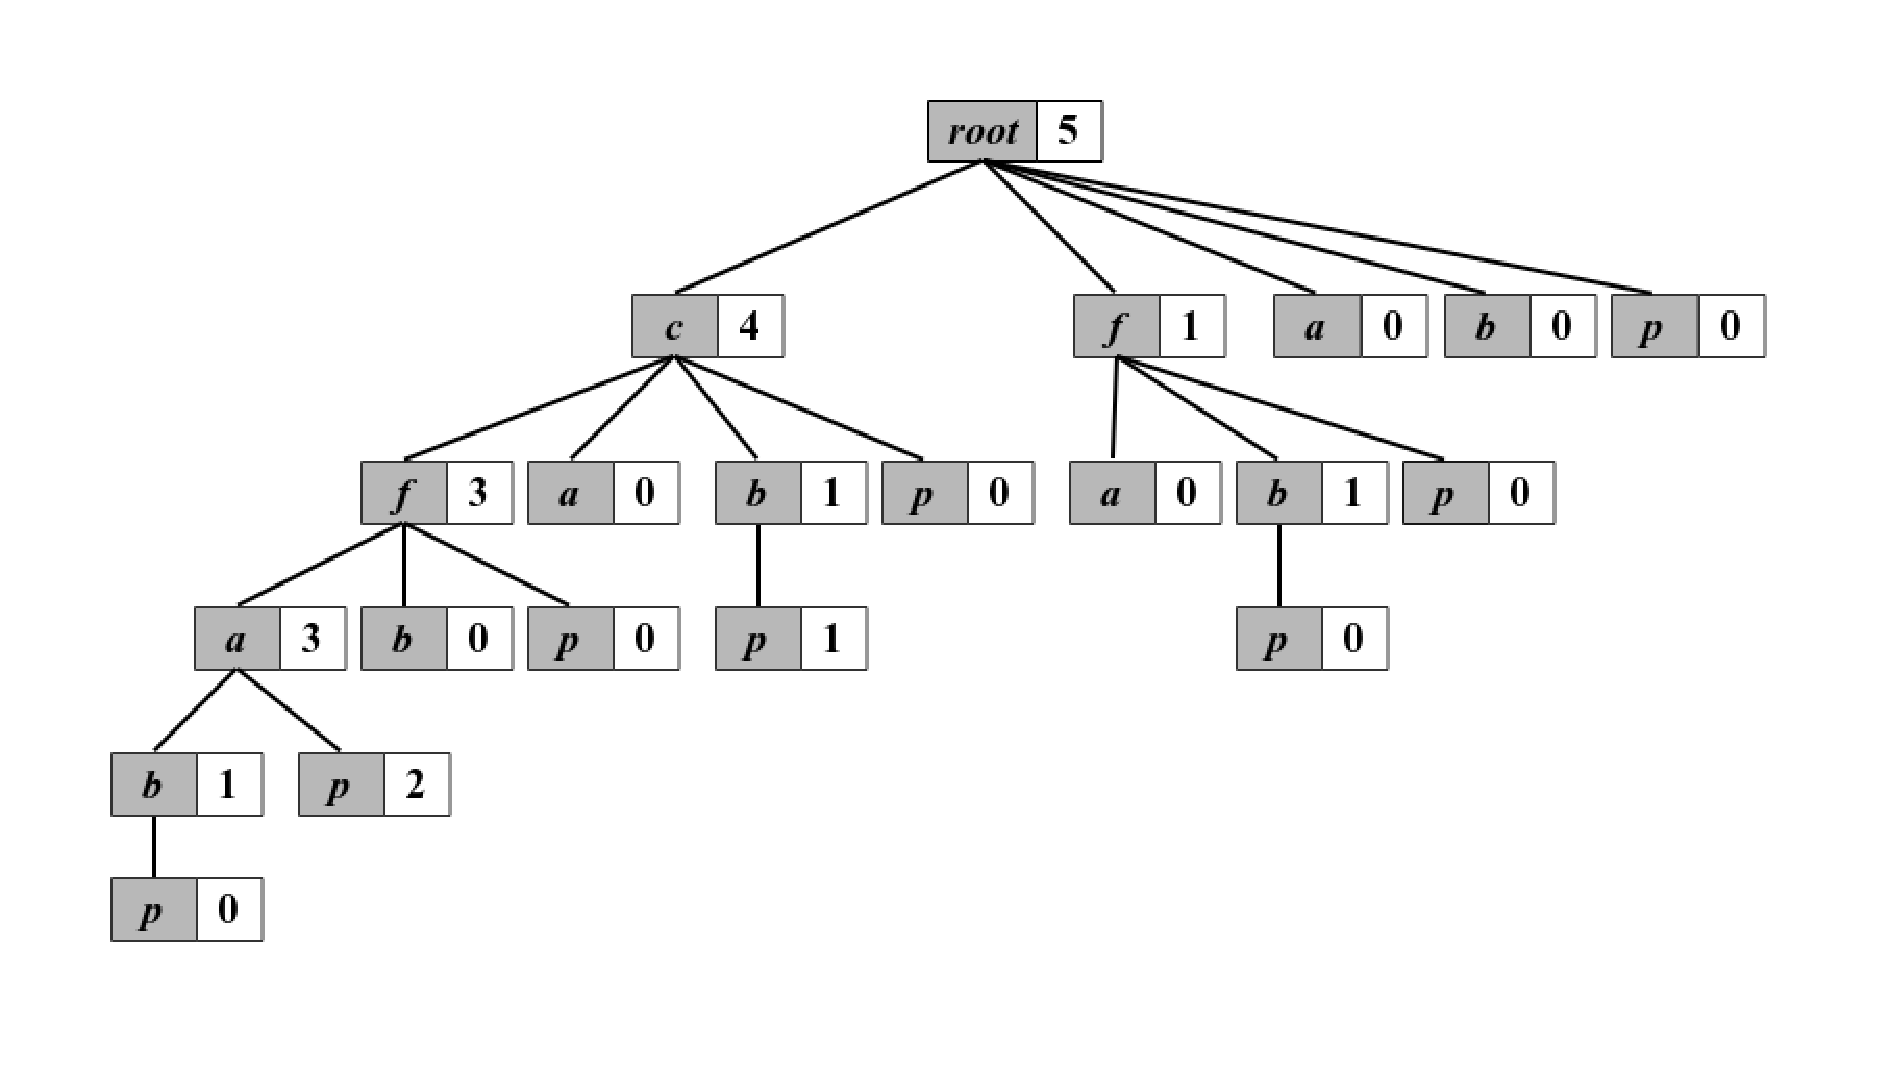
\includegraphics[width=0.8\textwidth]{123.pdf}
    \caption{模式树}
    \label{fig:fptree}
  \end{figure}

\subsection{minefp方案介绍}
\label{section:minefp}
根据上述对总体框架的介绍可知,本文主要工作是提出了minefp方案用以收集$top-k$的$\alpha -itemset(\alpha>1)$集合$\tilde{IS_k}$。

\begin{algorithm}[t]
    \caption{minefp}
    \label{alg:minefp}
        \begin{algorithmic}[1]
			 \REQUIRE ~~\\
			 数据集$DB_2$;\\
			 隐私预算$\epsilon$;\\
			 正整数$k$;\\
			 频繁$1-itemset$集合$\tilde{S_k}$;
			 \ENSURE $top-k$的挖掘结果$\tilde{IS_k}$

                 \STATE 预处理数据集$DB_2$,删除用户记录中的非频繁项目并重新排序; \\ //预处理数据集,$\tilde{S_k}$中的项目为频繁项目,并以其中项目顺序进行排序   
                 \label{minefp:preprocessing} 
                 %\STATE 分配隐私预算$\epsilon_1 + \epsilon_2 = \epsilon$;
                 %\label{minefp:epsilon}            
                 \STATE 将$DB_2$按比例分为互斥的两组$transaction_1$和$transaction_2$;
                 \label{minefp:group}
			 \STATE $iterNum = FO\_MaxIter(transaction_1,\epsilon)$; \\ //FO协议聚合transaction\_1中用户记录长度的信息,%详见算法\ref{alg:FO_MaxIter}
			 \label{minefp:iterNum}
			 \STATE $tree = build\_fpTree(transaction_2,\tilde{S_k},\epsilon,iterNum)$; \\ //层次构建频繁模式树,%详见算法\ref{alg:build_fpTree}
			 \label{minefp:tree}
			 \STATE $\tilde{IS} = FP\-growth(tree)$; \\ //FP-growth方法挖掘模式树tree
                 \label{minefp:fpgrowth}
			 \STATE 优化$\tilde{IS}$并选择$top-k$记为$\tilde{IS_k}$ \\ //后处理步骤,不消耗隐私预算
                 \label{minefp:optimize}
                 \RETURN $\tilde{IS_k}$
        \end{algorithmic}
\end{algorithm}

%对上述算法简单介绍,引出下文

算法\ref{alg:minefp}描述了minefp方案的总体框架,首先对整个用户数据进行预处理并分配隐私预算(步骤\ref{minefp:preprocessing}、\ref{minefp:group});然后为了建立频繁模式树,先聚合用户记录长度估计出树的最大层次(步骤\ref{minefp:iterNum}),最后以最大层次进行频繁模式树的层次建立(步骤\ref{minefp:tree});在建立模式树之后,挖掘出有效的频繁项集并且对结果进行一定的优化处理后发布(步骤\ref{minefp:fpgrowth}、\ref{minefp:optimize})。



%其中最主要是层次建立模式树tree(步骤\ref{minefp:tree})。

%步骤\ref{minefp:iterNum}是以LDP方式聚合得到树的最大层次iterNum,用于层次建树时更好的分配隐私预算,详见\ref{section:MaxIter}节;

%步骤\ref{minefp:tree}用于建立频繁模式树,详见\ref{section:buildTree}节;

%步骤\ref{minefp:fpgrowth}是FP-growth的挖掘方法,更多细节参见文献\cite{han2000mining};

%步骤\ref{minefp:optimize}为后处理步骤,用以优化最终发布结果,能够使结果更加准确。


\subsection{最大树层次}
\label{section:MaxIter}
由于本文是在LDP场景下层次建立频繁模式树,树的最大层次与隐私预算的分配直接相关。如图\ref{fig:fptree}所示模式树,最大层次为5。由于用户的记录长度也是敏感信息,其长度不固定且具有随机性。本文使用FO协议,聚合用户的记录长度,通过设置临界值$T=3.0 \cdot \frac{\sqrt{n}}{\epsilon}$,从而估计出有效的最大层次。

\begin{algorithm}[h]
\caption{FO\_MaxIter}
\label{alg:MaxIter}
\begin{algorithmic}[1]
\REQUIRE 数据集$transaction_1$;\\
隐私预算$\epsilon_1$;
\ENSURE 最大迭代次数MaxIter

\STATE 初始化临界值$T=3.0 \cdot \frac{\sqrt{n_1}}{\epsilon}$; //$n_1$为$transaction_1$的用户总数
\label{T threshold}
\STATE FO协议聚合用户记录长度,并且将长度人数不大于$T$的视作无效估计,置为0;

\STATE 利用公式(8)在$\gamma=0.8$时的整数值$M$;
\label{gamma=0.8}
\RETURN 最大迭代次数$M$
\end{algorithmic}
\end{algorithm}

 $$\varphi(X)=\prod_{x \in X} \mu(x) , \mu(x) = \frac{0.8\times \tilde{\theta}(x)}{\max \limits_{x \in S^{\prime}} \tilde{\theta}(x)}\eqno{(9)}$$

其过程与文献\cite{wang2018locally}中对$L$值的确定相似,本文对其中一些参数值做了修改,具体见算法\ref{alg:iter}。

\subsection{层次建树}
\label{section:buildTree}

%建树算法修改
\begin{algorithm}[htbp]
\caption{建树}
\label{alg:bulid tree}
\begin{algorithmic}[1]
\REQUIRE ~~\\
数据集$DB_2$;\\
隐私预算$\epsilon$;\\
正整数$k$;\\
频繁$1-itemset$集合$\tilde{S_k}$;
\ENSURE $\tilde{IS_k}$

\STATE 初始化树根结点$root$为空;
\STATE 初始化候选值域$I^{\prime}_{1}$为$S^{\prime}$中项目,作为第一层次的LDP聚合值域;
\STATE 将$D B^{\prime}_{3}$均分为$M$个人数相同的子组~~\\
$G_{1},G_{2},...,G_{M};$
\STATE 初始化FO协议标准差为$standard\_error$ ;

\FOR{层次$j=1$ to $M$}
    \STATE FO协议聚合$estimation = Aggregate(I^{\prime}_{j},j,G_{j})$;\\
    //用户使用前$level$个项目参与,若无记录,则以无效值$\perp$参与。
    \STATE 删除$estimation$中估计值不大于$standard\_error$的结果;\\
    //无效值$\perp$不用于建树。
    \STATE 以$estimation$聚合结果更新第$j$层树$root$节点;
    \STATE 根据第$j$层节点,生成所有可能的孩子节点,作为下一层初始值域$I_{j+1}$;
    %\STATE $I^{\prime}_{j+1} = \text{算法\ref{alg:prune}}(I_{j+1},S^{\prime},k,\xi)$
\ENDFOR

\RETURN $root$
\end{algorithmic}
\end{algorithm}

\section{结果优化}
\label{section:optimize}

\section{实验}

\end{document}